\documentclass[]{article}
\usepackage[utf8]{inputenc}
\usepackage{amsmath}
\usepackage{amsfonts}
\usepackage{amssymb}
\usepackage{graphicx}

\title{Reporte 7 [Mareas]}
\author{Antonio Cota Rodr\'iguez}
\date{}

\begin{document}
\maketitle

\section*{Introducci\'on}
La marea es el cambio periódico del nivel del mar producido principalmente por la fuerza de atracción gravitatoria que ejercen el Sol y la Luna sobre la Tierra. Aunque dicha atracción se ejerce sobre todo el planeta, tanto en su parte sólida como líquida y gaseosa, nos referiremos en este artículo a la atracción de la Luna y el Sol, juntos o por separado, sobre las aguas de los mares y océanos. Sin embargo, hay que indicar que las mareas de la litosfera son prácticamente insignificantes, con respecto a las que ocurren en el mar u océano (que pueden modificar su nivel en varios metros) y, sobre todo, en la atmósfera, donde puede variar en varios km de altura, aunque en este caso, es mucho mayor el aumento del espesor de la atmósfera producido por la fuerza centrífuga del movimiento de rotación en la zona ecuatorial (donde el espesor de la atmósfera es mucho mayor) que la modificación introducida por las mareas en dicha zona ecuatorial.
Periodo_mensual_max
Otros fenómenos ocasionales, como los vientos, las lluvias, el desborde de ríos y los tsunamis provocan variaciones del nivel del mar, también ocasionales, pero no pueden ser calificados de mareas, pero que no están causados por la fuerza gravitatoria.

\section*{Series de tiempo}
Una serie de tiempo es una secuencia de puntos datos, medidos t\'ipicamente
en puntos sucesivos en el tiempo espaciados en intervalos de tiempos uni-
formes. Normalmente estas se representan con mucha frecuencia a trav\'es de
los gr\'aficos de l\'ineas. Las series temporales se utilizan en las estad\'isticas, procesamiento de señales, reconocimiento de patrones, la econometr\'ia, finanzas matem\'aticas, la predicci\'on del tiempo, la predicci\'on de terremotos, electroencefalograf ́ıa, la ingenier\'ia de control, la astronom\'ia y la ingenier\'ia
de comunicaciones.


\section*{Teor\'ia de las mareas}

La teor\'ia din\'amica de las mareas describe y predice el comportamiento real de las olas en los oc\'eanos.
Mientras que Newton explicaba las mareas describiendo una fuerza generadora de las mareas y Bernoulli dio una descrpci\'on de la reacci\'on est\'atica del agua en la Tierra al potencial de marea, la teor\'ia din\'amica de las mareas, desarrollada por Pierre-Simon Laplace describe la reacci\'on real a las fuerzas de marea del oc\'eano. La teor\'ia de Laplace de los mareas de los oc\'eanos toma en cuenta la fricci\'on, resonancia y los periodos naturales de las cuencas oce\'anicas.

\section*{Componentes de las mareas}

Los cambios de las mareas son el resultado neto de m ́ultiples influencias que

act\'uan sobre diferentes per\'iodos. Estas influencias se denominan compo-
nentes de la marea. Los principales son la rotaci\'on de la Tierra, las posiciones
de la Luna y el Sol respecto a la Tierra, la altitud de la Luna (elevaci\'on) so-
bre el ecuador de la Tierra, y la batimetr\'ia (el equivalente oce\'<nico de la topograf\'ia). Estos componentes determinan las frecuencias de los arm\'onicos, es decir que existe una estrecha relaci ́on con los ciclos de las fuerzas astron ́omicas, mencionadas anteriormente.
\\\\\\
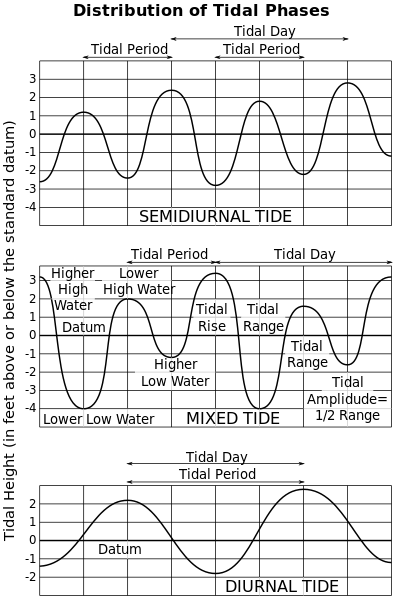
\includegraphics[scale=0.5]{Tides}


\section*{C\'odigo de Fortran}

A continuaci\'on se brindar\'a el c\'odigo para Fortran.

\begin{verbatim}

PROGRAM Mareas

IMPLICIT NONE

! Declaracion de variables 1

REAL, DIMENSION (7674):: altura
INTEGER :: i

! Declaracion de variables 2

real :: M1, M2, M3, M4, M5, Dif    ! Maximox
real :: T1, T2, T3, T4, T5 ! Tiempom#x
real :: Dif2, E1Min, E2Min, E3Min, E4Min, E5Min !Minm#
real :: T1n, T2n, T3n, T4n, T5n !Tiempon
real :: Dif3, d1Mx, d2Mx, d3Mx, d4Mx, d5Mx !Maxd#
real :: T1x, T2x, T3x, T4x, T5x !Tiempod#x
real :: Dif4, F1Mi, F2Mi, F3Mi, F4Mi, F5Mi !Mind#
real :: E1nT, E2nT, E3nT, E4nT, E5nT !Tiempod#n
real :: PM1, PM2, PM3, PM4, PM5 !PeriodomM#
REAL :: PN1, PN2, PN3, PN4, PN5 !PeriodomN#
REAL :: PdM1, PdM2, PdM3, PdM4, PdM5 !PeriododM#
REAL :: PdN1, PdN2, PdN3, PdN4, PdN5 !PeriododN#
REAL :: Mensual_maximo !Periodo_mensual_max
REAL :: Mensual_minimo !Periodo_mensual_min
REAL :: Diario_max !Periodo_diario_max
REAL :: Diario_min !Periodo_diario_min





OPEN (1,file="Mareas.csv")

DO i=1,7674
READ (1,*) altura(i)
END DO
CLOSE (1)
!*************************************
M1 = 0
DO i=1,1344
Dif=M1 - altura(i)
IF (Dif < 0) THEN 
M1 = altura (i)

T1= i/48.0

END IF
END DO

!************************************

M2 = 0
DO i=1345,2690
Dif =  M2 - altura(i)
IF (Dif < 0) THEN 
M2 = altura(i)

T2=i/48.0
END IF
END DO

!************************************

M3 = 0
DO i=2691,4035
Dif = M3 - altura(i)
IF (Dif < 0) THEN 
M3 = altura (i)

T3=i/48.0
END IF
END DO 

!************************************

M4 = 0
DO i=4036,5380
Dif = M4 - altura(i)
IF (Dif < 0) THEN 
M4 = altura (i)

T4=i/48.0
END IF
END DO

!************************************

M5 = 0
DO i=5381, 6725
Dif = M5 - altura(i)
IF (Dif < 0) THEN 
M5 = altura (i)

T5=i/48.0
END IF
END DO

!************************************

E1Min = 0
DO i= 1, 1344
Dif2= E1Min - altura(i)
IF (Dif2> 0) THEN 
E1Min = altura (i)

T1n=i/48.0
END IF
END DO

!************************************

E2Min = 0
DO i= 1345, 2690
Dif2= E2Min - altura(i)
IF (Dif2> 0) THEN 
E2Min = altura (i)

T2n=i/48.0
END IF
END DO

!************************************

E3Min = 0
DO i= 2691, 4035
Dif2= E3Min - altura(i)
IF (Dif2> 0) THEN 
E3Min = altura (i)

T3n=i/48.0
END IF
END DO

!************************************

E4Min = 0
DO i= 4036, 5380
Dif2= E4Min - altura(i)
IF (Dif2> 0) THEN 
E4Min = altura (i)

T4n=i/48.0
END IF
END DO

!************************************

E5Min = 0
DO i= 5381, 6725
Dif2= E5Min - altura(i)
IF (Dif2> 0) THEN 
E5Min = altura (i)

T5n=i/48.0
END IF
END DO


!************************************

d1Mx = 0
DO i= 18, 65
Dif3= d1Mx- altura(i)
IF (Dif3< 0) THEN 
d1Mx = altura (i)

T1x= i * 0.5

END IF
END DO

!************************************

d2Mx = 0
DO i= 66, 113
Dif2=  d2Mx - altura(i)
IF (Dif3< 0) THEN 
d2Mx = altura(i)

T2x=(i* 0.5)

END IF
END DO

!************************************

d3Mx = 0
DO i= 114, 161
Dif3= d3Mx - altura(i)
IF (Dif3< 0) THEN 
d3Mx = altura (i)

T3x=(i* 0.5)

END IF
END DO 

!************************************

d4Mx = 0
DO i= 162, 209
Dif3= d4Mx - altura(i)
IF (Dif3< 0) THEN 
d4Mx = altura (i)

T4x=(i* 0.5)

END IF
END DO 

!************************************

d5Mx = 0
DO i= 210, 257
Dif3= d5Mx - altura(i)
IF (Dif3< 0) THEN 
d5Mx = altura (i)

T5x=(i* 0.5)

End if
End do 

!************************************---------------------

F1Mi = 0
DO i= 18, 65
Dif4= F1Mi - altura(i)
IF (Dif4> 0) THEN 
F1Mi = altura (i)

E1nT=i * 0.5

END IF
END DO

F2Mi = 0
DO i= 66, 113
Dif4= F2Mi - altura(i)
IF (Dif2> 0) THEN 
F2Mi = altura (i)

E2nT=( i * 0.5) 
END IF
END DO

F3Mi = 0
DO i= 114, 161
Dif4= F3Mi - altura(i)
IF (Dif4> 0) THEN 
F3Mi = altura (i)

E3nT=(i* 0.5) 

END IF
END DO

F4Mi = 0
DO i= 162, 209
Dif4= F4Mi - altura(i)
IF (Dif4> 0) THEN 
F4Mi = altura (i)

E4nT=(i* 0.5) 

END IF
END DO

F5Mi = 0
DO i= 210, 257
Dif4= F5Mi - altura(i)
IF (Dif4> 0) THEN 
F5Mi = altura (i)

E5nT=(i* 0.5) 

END IF
END DO
!--------------------------------------------

PM1 = T1x 
PM2 = T2x - T1x
PM3 = T3x - T2x
PM4 = T4x - T3x
PM5 = T5x - T4x

PN1 = T1n 
PN2 = T2n - T1n
PN3 = T3n - T2n
PN4 = T4n - T3n
PN5 = T5n - T4n

PdM1 = T1x 
PdM2 = T2x - T1x
PdM3 = T3x - T2x
PdM4 = T4x - T3x
PdM5 = T5x - T4x

PdN1 = E1nT 
PdN2 = E2nT - E1nT
PdN3 = E3nT - E2nT
PdN4 = E4nT - E3nT
PdN5 = E5nT - E4nT

!---------------------------------------------

Mensual_maximo = (PM1 + PM2 + PM3 + PM4 + PM5)/5.0

Mensual_minimo = (PN1 + PN2 + PN3 + PN4 + PN5)/5.0

Diario_max = (PdM1 +PdM2 +PdM3 + PdM4 + PdM5)/5.0

Diario_min = (PdN1 +PdN2 +PdN3 + PdN4 + PdN5)/5.0




Print *, 'Mensualmente las mareas maximas fueron de:'       
Print *, 'Primer mes:', M1,'En el dia:', T1
Print *, 'Segundo mes:',M2,'En el dia:', T2              
Print *, 'Tercer mes:',M3,'En el dia:', T3
Print *, 'Cuarto  mes:',M4,'En el dia:', T4             
Print *, 'Quinto mes:',M5,'En el dia:', T5

!-
Print *, 'Mensualemte las mareas minimas fueron:'
       
Print *, 'Primer mes:',E1Min, 'En el dia:', T1n
Print *, 'Segundo mes:',E2Min,'En el dia:', T2n           
Print *, 'Tercer mes:',E3Min,'En el dia:', T3n
Print *, 'Cuarto  mes:',E4Min,'En el dia:', T4n              
Print *, 'Quinto  mes:',E5Min,'En el dia:', T5n

Print *, 'El periodo de marea maxima es:', Mensual_maximo, 'dias'

Print *, 'El periodo de marea minima es:', Mensual_minimo, 'dias'

Print *, 'Las mareas maximas diarias fueron:'       
Print *, 'Primer dia:', d1Mx
Print *, 'Segundo dia:',d2Mx           
Print *, 'Tercer dia:',d3Mx
Print *, 'Cuarto dia:',d4Mx           
Print *, 'Quinto dia:',d5Mx

Print *, 'Las mareas minimas diarias fueron:'     

Print *, 'Primer dia:',F1Mi
Print *, 'Segundo dia:',F2Mi             
Print *, 'Tercer dia:',F3Mi
Print *, 'Cuarto dia:',F4Mi              
Print *, 'Quinto dia:',F5Mi


Print *, 'El periodo diario de la marea maxima es:', Diario_max, 'hrs'

Print *, 'El periodo diario de la marea  minima es:', Diario_min, 'hrs' 



end program Mareas


\end{verbatim}

\section*{An\'alisis de datos}
La siguiente imagen muestra los datos que se utilizar\'an para describir la variaci\'on del nivel del agua respecto al tiempo durante lo que dur\'o el experimento.

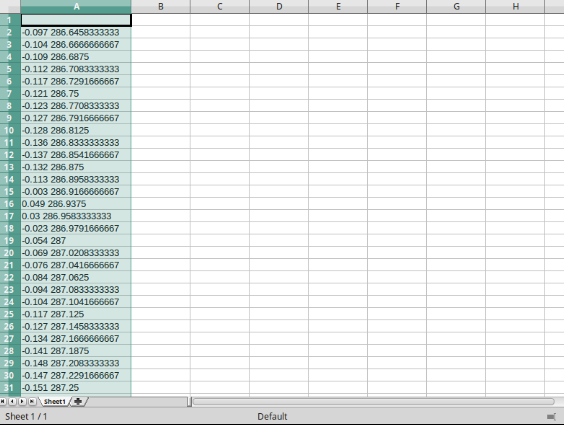
\includegraphics[scale=0.5]{Datos}\\

A continuaci\'on se muestra una imagen de los datos proporcionados por el programa en Fortran. 

\begin{center}
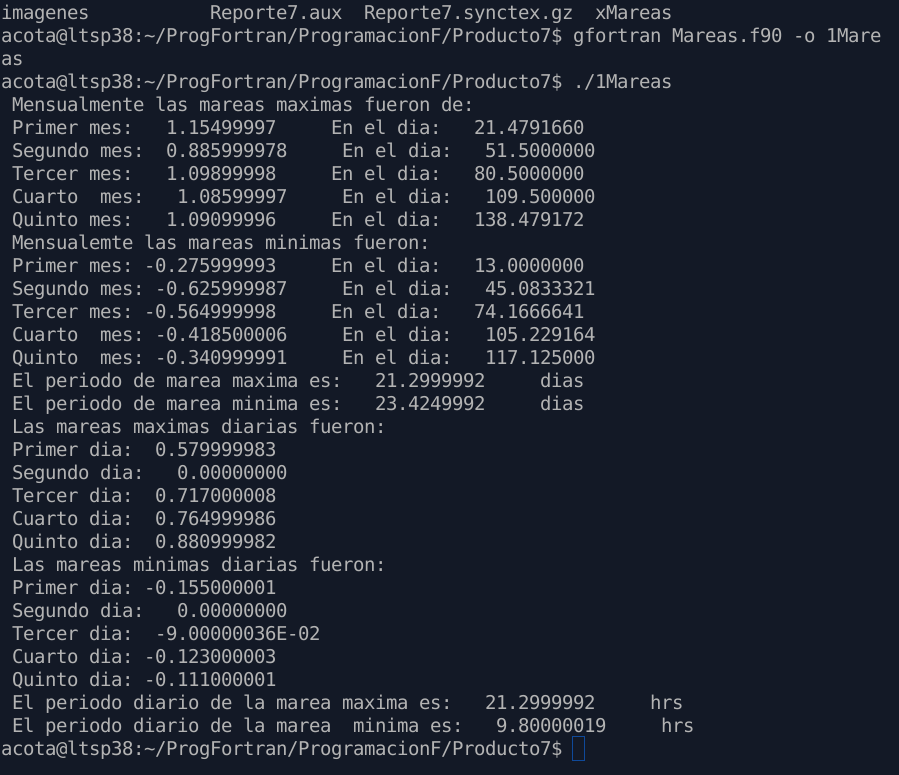
\includegraphics[scale=0.5]{Mareainfo}\\

\end{center}



Al utilizar todos estos datos y el programa 'gnuplot' pasamos a graficar, con unos ejes adecuados queda de la siguiente manera:
\begin{center}
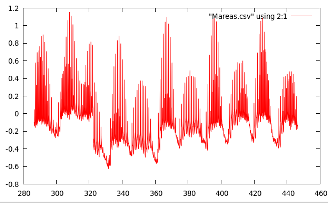
\includegraphics[scale=1]{GraficaMareas}
\end{center}


\end{document}